 \documentclass[12pt]{article}
\usepackage[T2A]{fontenc}
\usepackage[utf8]{inputenc}       

\usepackage[english]{babel}
\usepackage{amsmath,amsfonts,amsthm,amssymb,amsbsy,amstext,amscd,amsxtra,multicol}
\usepackage{verbatim}
\usepackage{tikz}
\usetikzlibrary{automata,positioning}
\usepackage{multicol}
\usepackage{graphicx}
\usepackage[colorlinks,urlcolor=blue]{hyperref}
\usepackage[stable]{footmisc}
\usepackage{ dsfont }
\usepackage{wrapfig}
\usepackage{xparse}
\usepackage{ifthen}
\usepackage{bm}
\usepackage{color}
 \usepackage{subfigure}
 
\usepackage{algorithm}
\usepackage{algpseudocode}

\usepackage{xcolor}
\usepackage{hyperref}
\definecolor{linkcolor}{HTML}{799B03} % цвет гиперссылок
\definecolor{urlcolor}{HTML}{799B03} % цвет гиперссылок
 
%\hypersetup{pdfstartview=FitH,  linkcolor=linkcolor,urlcolor=urlcolor, colorlinks=true}

\newtheorem{theorem}{Theorem}[section]
\newtheorem{lemma}{Lemma}[section]

\DeclareMathOperator{\sign}{sign}
\DeclareMathOperator{\grad}{grad}
\DeclareMathOperator{\intt}{int}
\DeclareMathOperator{\conv}{conv}
\begin{document}

\tableofcontents
\newpage

\section{Introduction}

In this paper we research one method of optimization on a square in $\mathbb{R}^2$. The method was offered by Nesterov (see ex.~4 from ~\cite{task}). 

In the paper~\cite{Ston_Pas} there are some results for this method. Namely, there are some estimates for iterations number and accuracy for task on segment (see the next section or \cite{Ston_Pas}). Also there are comparison of this method with method of ellipsoids. Discussed method showed better results on time.

In this paper we want to continue this research. In the next section there is description of method and pseudocode for it. In the section~3. there are results where this method works correctly. The section~4. includes two ways to estimate accuracy for a task on segment and it is one of two main results in this paper. Following important result is theorem 5.3 for iterations number that is asymptotically twice as good as the estimate in \cite{Ston_Pas}.

Section Tests include different tests that show some theoretical results in practice and include comparison of this method with gradient descent. 

\section{Method Description}

Let's consider a following task:

$$\min_{(x,y)}\left\{f(x,y)|(x,y) \in Q\right\},$$
where $f$ is a convex function, $Q$ - is a square on the plane.

Let's consider a following method. One solves task of minimization for a function $g(x) = f\left(x, y_0 = \frac{a}{2}\right)$ on a segment $[0, a]$ with an accuracy $\delta$ on function. After that one calculates a sub-gradient in a received point and chooses the rectangle which the sub-gradient "does not look" in. Similar actions are repeated for a vertical segment. As a result we have the square decreased twice. Let's find a possible value of error $\delta_0$ for task on segment and a sufficient iteration's number $N$ to solve the initial task with accuracy $\epsilon$ on function.

Let's describe an algorithm formally. See pseudo-code \ref{alg:Example}.

\begin{algorithm}[H]
\caption{Algorithm of the method}\label{alg:Example}
\begin{algorithmic}[1]
\Function{Method}{convex function $f$, square $Q = [a, b]\times[c,d]$}

$x_0:= solve(g = f(\cdot, \frac{c+d}{2}), [a,b], \delta)$
 
$g = subgradient(f, (x_0, \frac{c+d}{2}))$
 
\If{g[1] > 0}
\State$Q := [a,b] \times [c, \frac{c+d}{2}]$ 
\Else
\State$Q := [a,b] \times [\frac{c+d}{2}, d]$ 
\EndIf

 $y_0:= solve(g = f(\frac{a+b}{2}, \cdot), [c,d], \delta)$
 
 $g := subgradient(f, (\frac{a+b}{2}), y_0)$
 
 \If{g[0] > 0}
 \State$Q := [a, \frac{a+b}{2}] \times [c, d]$ 
\Else
\State$Q := [\frac{a+b}{2},b] \times [c, d]$ 
\EndIf
\If{StopRec() == False}
\State Method($f$, $Q$) 
\EndIf
\Return $(\frac{a+b}{2}, \frac{c+d}{2})$
\EndFunction 
 \end{algorithmic}
\end{algorithm}

\section{Algorithm correctness}
Let's $\textbf{x}_0$ is solution of the task on segment, $Q_1$ is choosed rectangle, $Q_2$ is not choosed rectangle.

\subsection{Zero Error}

\begin{lemma}\label{l1}
If the optimization task on segment is solved with zero error and the $f$ is convex and differentiable at a point-solution, rectangle with solution of initial task was choosed correct.
\end{lemma}
\begin{proof}
From sub-gradient definition, $\textbf{x}^* \in \{x|(\textbf{g}(\textbf{x}_0), \textbf{x}_0 - \textbf{x}^*) \geq 0)\}$. Lemma's statement follows from it and a fact that the first (or the second for vertical segment) gradient's component in point $\textbf{x}_0$ is zero.
\end{proof}


\subsection{Nonzero Error}
\begin{theorem}
Let's the $f$ has continuous derivative on the square. Then there is a neighbourhood of a solution of optimization task on segment such as a choice of rectangle will not change if one use any point from the   neighbourhood.
\end{theorem}
\begin{proof}
Let's consider a case when we work with horizontal segment. Case with vertical segment is considered analogously. Then we are interesting in $f_y'(x_0, y_0)$. If $\textbf{x}_0$ is not solution of initial task, then $f_y'(x_0, y_0) \neq 0$. 

From a continuity of the derivative:

$$\lim\limits_{\delta \rightarrow 0}f_y'(x_0+\delta, y_0) = f_y'(x_0, y_0)$$

Therefore, 

$$\exists \delta_0:\forall \textbf{x}_\delta\in B_{\delta_0}(x_0)\times y_0\Rightarrow \sign(f_y'(\textbf{x}_\delta)) = \sign(f_y'(\textbf{x}_0))$$

From it and lemma 4.1 theorem's statement follows.

\end{proof}

\subsection{Undifferentiable convex function}

The method does not work for all convex functions even for zero error on segment. 

\textbf{Example 1.} There is an example in \cite{Ston_Pas}.

\section{Error's Value}

From derivative continuously we have following obvious result:

\begin{lemma}
If $f$ has continuous derivative. If $|f'_y(x, y_0)| > 0$ for all $x$ on horizontal segment, then the second gradient's component has same sign at all points of segment. If $|f'_x(x_0, y)| > 0$ for all $y$ on vertical segment, then the first gradient's component has same sign at all points of segment.
\end{lemma}

\textbf{Example 2.} All functions $f$ of the following type meet conditions of written above lemma:

$$f(x, y) = \psi(x) + \phi(y),$$
where $\psi, \phi$ are convex and differentiable functions.

\textbf{Example 3.} Let's illustrate that we can not always take any point from segment. Let's consider following task:

$$\min\left\{(x-y)^2 + x^2\Big|Q = [0,1]^2\right\}$$

On segment $[0,1]\times\left\{\frac{1}{2}\right\}$ this task has solution $f^* = f\left(\frac{1}{4}, \frac{1}{2}\right) = \frac{1}{8}$. Derivative on $y$ at this point is $f'_y\left(\frac{1}{4}, \frac{1}{2}\right) = \frac{]}{2}$ but at the point $\left(1, \frac{1}{2}\right)$ is equal to $-1$. We can see that in this case rectangle will selected non-correctly.

Let's find possible value of error's value, i.e. let's find a number $\delta_0$ such as if an error for   a solution on a segment is less $\delta_0$ then rectangle for the segment is defined correctly. Rectangles are defined correctly for a horizontal optimization task, if:

\begin{equation}\label{MCH}
\forall\delta : |\delta| < \delta_0 \Rightarrow f'_y(\textbf{x}_0)f'_y(x_0+\delta, y_0) > 0
\end{equation}

Analogically, for a vertical segment:
\begin{equation}\label{MCV}
\forall\delta: |\delta| < \delta_0 \Rightarrow f'_x(\textbf{x}_0)f'_x(x_0, y_0+\delta) > 0
\end{equation}




\begin{theorem}
\label{ConstGrad}
Let function $f$ be convex and has $L$-Lipschitz continuous gradient and a point $\textbf{x}_0$ is a solution of optimization's  task on a current segment. 

The current segment is horizontal and $\exists M>0  : \Rightarrow|f_y'(\textbf{x}_0)| \geq M$ or the current segment is vertical and $\exists M>0  : \Rightarrow|f_x'(\textbf{x}_0)| \geq M$. Then rectangle is defined correctly if the possible value of error is less than $\frac{M}{L}$.
\end{theorem}
\begin{proof}
Condition \eqref{MCH} is met if there is a derivative $f'_y(x_0+\delta, y_0)$ in a neighbourhood of 
$f'_y(\textbf{x}_0)$ with radius $\left|f'_y(\textbf{x}_0)\right|$:

$$\left|f'_y(\textbf{x}_0) - f'_y(x_0+\delta, y_0)\right|<\left|f'_y(\textbf{x}_0)\right|$$

The $L$-Lipschitz continuity gives following inequality:

$$\left|f'_y(\textbf{x}_0) - f'_y(x_0+\delta, y_0)\right| \leq L|\delta|$$

Therefore the following possible value is sufficient to select rectangle correctly:

$$\delta_0 < \frac{M}{L} \leq \frac{\left|f'_y(\textbf{x}_0)\right|}{L}$$

Statement for vertical segment is proved similarly.
\end{proof}

In written above theorem the estimate needs some lower bound for derivatibe in point-solution on segment and this task can be hard in practise. Using other interpretation of the condition \eqref{MCH} one can take more useful result.

\begin{theorem}
\label{CurGrad}
Let function $f$ be convex and has $L$-Lipschitz continuous gradient and a point $\textbf{x}_0$ is a solution of optimization's  task on a current segment. 

The current segment is horizontal and $M = |f_y'(\textbf{x}_{current})|$ or the current segment is vertical and $M = |f_y'(\textbf{x}_{current})|$. Then rectangle is defined correctly if a distance between $\textbf{x}_{cur}$ and accurate solution on segment is less than $\frac{M}{L}$.
\end{theorem}
\begin{proof}
Condition \eqref{MCH} is met if there is a derivative $f'_y(x_0+\delta, y_0)$ in a neighbourhood of 
$f'_y(\textbf{x}_0)$ with radius $\left|f'_y(\textbf{x}_{cur})\right|$:

$$\left|f'_y(\textbf{x}_0) - f'_y(\textbf{x}_{cur})\right|<\left|f'_y(\textbf{x}_{cur})\right|$$

The $L$-Lipschitz continuity gives following inequality:

$$\left|f'_y(\textbf{x}_0) - f'_y(\textbf{x}_{cur})\right| \leq L|\delta|$$

Therefore the following possible value is sufficient to select rectangle correctly:

$$\delta_0 < \frac{M}{L} \leq \frac{\left|f'_y(\textbf{x}_0)\right|}{L}$$

Statement for vertical segment is proved similarly.
\end{proof}

Theorems 4.1 and 4.2 give stop conditions in the case when gradient in point-solution on segment and close points is large. But what should we do if gradient in this point is small?

\begin{theorem}
Let $f$ be convex and has $L$-Lipschitz continuous gradient. Then for accuracy on function $\epsilon$ following condition in point $\textbf{x}$ is sufficient:

$$\|\nabla f(\textbf{x})\|\leq \frac{\epsilon}{a\sqrt{2}}, $$
where $a$ is size of current square.
\end{theorem}

\begin{proof}
Let's consider following inequality for convex functions (see prove in \cite{Nesterov}):

$$f(\textbf{x}^*) - f(\textbf{x}) \geq (\nabla f(\textbf{x}), \textbf{x}^* - \textbf{x} )$$

Using  Cauchy–Bunyakovsky–Schwarz inequality one has following inequality

$$f(\textbf{x}) - f(\textbf{x}^*) \leq -(\nabla f(\textbf{x}), \textbf{x}^* - \textbf{x} )\leq$$
$$\leq \|\nabla f(\textbf{x})\| \|\textbf{x}^* - \textbf{x}\|\leq \|\nabla f(\textbf{x})\|a\sqrt{2}$$

This inequality proves theorem's statement.
\end{proof}

Let's make a couple of remarks.

Firstly, we can replace the Lipschitz condition on the square by the Lipschitz condition on the segments in the theorems 4.1 and 4.2.

Thirdly, all theorems in this section use $f'_y$ on horizontal segment and $f'_x$ on vertical segment. As a result, if one checks condition of stop on each iteration method will use full gradient on each iteration. It can slow down method but this estimates can be better than in ~\cite{Ston_Pas}. As a result, method can work faster.

\section{Number of iterations}

Below proved estimates are correct if each iterations was correct, i.e. after each iteration there is the solution in the selected rectangle. It is important condition

\begin{theorem}
If function $f$ is convex and $L_f$-Lipschitz continuous, then for to solve initial task with accuracy $\epsilon$ on function one should make following iteration's numbers:
\begin{equation}\label{NI1}N = \left\lceil\log_2\frac{\sqrt{2}L_fa}{\epsilon}\right\rceil\end{equation}
where $a$ is a size of the initial square $Q$.
\end{theorem}

This estimate is trivial consequence of the function is Lipschitz continuous.

There are functions which estimates from written above theorem are very accurate for.

\textbf{Example 5.} Let's consider following task with positive constant $A$:

$$\min\left\{A(x+y)|Q = [0,1]^2\right\}$$

If one take a center of a current solution as approximate  solution one have value $\frac{A}{2^N}$ after $N$ iterations. Therefore, for accuracy $\epsilon$ one has to $\lceil\log_2\frac{A}{\epsilon}\rceil$. For this function $L_f = 2A$. Therefore, estimate \eqref{NI1} is accurate for such tasks with little error that not more one iteration.

But any convex function is locally Lipschitz continuous at all $x \in \intt Q$. Therefore, we have following theorem.

\begin{theorem}
If function $f$ is convex and a solution $x^*\in \intt Q$, then for to solve initial task with accuracy $\epsilon$ on function one has to take a center of a current square as approximate  solution and make following iteration's numbers:
\begin{equation}\label{NI2}
N = \left\lceil\log_2\max\left\{\frac{a}{\epsilon_0(\textbf{x}^*)},\frac{\sqrt{2}L_fa}{\epsilon}\right\}\right\rceil
\end{equation}
where $a$ is a size of the initial square $Q$, $\epsilon_0(x^*)$ is size of neighbourhood of $x^*$ which $f$ is $L_f$-Lipschitz continuous in, $\Delta f =  f(x_0) - f(x^*)$, $x_0$ is a center of square $Q$.
\end{theorem}

We can improve written above estimates if to add new conditions:

\begin{theorem}
Let function $f$ be convex and has $L$-Lipschitz continuous gradient.

If solution is a internal point, then for to solve initial task with accuracy $\epsilon$ on function one should make following iteration's numbers:
\begin{equation}\label{NI3}N = \left\lceil\frac{1}{2}\log_2\frac{La^2}{2\epsilon}\right\rceil\end{equation}
where $a$ is a size of the initial square $Q$.
\end{theorem}

\begin{proof}
For all convex functions there is following inequality (one may find proof in \cite{Nesterov}):
$$f(\textbf{x}) - f(\textbf{x}^*) - (f'(\textbf{x}^*), \textbf{x} - \textbf{x}^*) \leq \frac{L}{2}\|\textbf{x}-\textbf{x}^*\|^2$$

If $\textbf{x}^*$ is a solution and an internal point, then $f'(\textbf{x}^*) = 0$:

$$f(\textbf{x}) - f(\textbf{x}^*)\leq \frac{L}{2}\|\textbf{x}-\textbf{x}^*\|^2$$

After $N$ iterations we have the estimate:

$$f(\textbf{x}) - f(\textbf{x}^*)\leq \frac{L}{4}\left(\frac{a}{2^N}\right)^2$$

Using it we have estimate \eqref{NI3}.
\end{proof}

Estimate \ref{NI1} works in all cases and better then estimate \ref{NI3} when following condition is met:

$$\frac{2L_f^2}{L_g}\leq \epsilon,$$
где $L_f, L_g$ is Lipschitz constants for function and for gradient. On the other hand, the estimate \ref{NI3} works if point with zero gradient exists in the square. 

\section{Details}
\label{details}
\subsection{Function Parameters}

This method was created to solve dual task. Namely, following task:

\begin{gather}
-\phi(\lambda_1, \lambda_2) \rightarrow \min_{\lambda\geq 0},\\
\text{where } \phi = \min_\textbf{x}\left(f(\textbf{x}) + \lambda_1 g_1(\textbf{x}) + \lambda_2 g_2(\textbf{x})\right)
\end{gather}

In the section we will discuss how transform this task to task of the task of minimization on square, what is derivative and lipschitz constants and how to calculate its fastly.

Fitstly, let's transform this task to the task of minimization on square. According to \cite{task} (see ex. 4.1), we can add following restraint for the dual variables:

\begin{gather}
\label{restr:dual}
\|{\lambda}\|_1 \leq \lambda_{\text{max}} = \frac{1}{\gamma}\left(f(\overline{\textbf{x}}) -\min\limits_{\textbf{x}}f(\textbf{x})\right),\\
\text{where $\overline{\textbf{x}}:g_i(\overline{\textbf{x}})<0,\gamma = \min\limits_ig_i(\overline{\textbf{x}})$}
\end{gather}
And we understand that there is the dual task's solution in a square $Q = [0, \lambda_{\text{max}}]^2$. And we have following optimization task:
\begin{gather}
\label{dual}
-\phi(\lambda_1, \lambda_2) \rightarrow \min_{\lambda \in Q}
\end{gather}

Secondly, the gradient of function $\phi$ will be calculated according well-known Demyanov-Danskin-Rubinov Theorem, see \cite{DDR-theorem}.

\begin{theorem}
Let $\phi(\lambda)=\min\limits_{x\in X}\Phi(x,\lambda)$ for all $\lambda\geq0$, where $\Phi$ is a smooth convex function with respect to $\lambda$ and $x(\lambda)$ is the only maximum point. Then
$$\nabla \phi(\lambda) = F'_\lambda\left(x(\lambda),\lambda\right)$$
\end{theorem}

If theorem's conditions is met for our case then we have derivative value:

\begin{equation}
\phi'_{\lambda_k}(\lambda) = g_k\left(\textbf{x}(\lambda)\right)
\end{equation}

Additionally, we need a Lipschitz constant for gradient. In the work \cite{Stonykin} there is following theorem:
\begin{theorem}
Let $f(x)$ be a $\mu_f$-strongly convex function, the function $g(x)$ satisfies the Lipschitz condition with a constant $M_g$. Then the function $\phi(\lambda) = \min_\textbf{x}\left(f(\textbf{x}+\lambda_1g_1(\textbf{x}) + \lambda_2g_2(\textbf{x})\right)$ defined in \ref{phi}, where $x(\lambda) = \arg\min\limits_x(f(x)+\lambda g(x))$, has Lipschitz smooth gradient with constant $L_{\phi'} = \frac{M_g^2}{\mu_f}$
\end{theorem}

This theorem can be proved easy for the 2-dimensional space. In this case $g$ is a vector-function.

In the following subsection we can use following notations:

$$\Phi(\textbf{x},\lambda) = f(\textbf{x}) + \lambda_1g_1(\textbf{x}) + \lambda_2g_2(\textbf{x})$$
$$\textbf{x}(\lambda) = \arg\min_\textbf{x}\Phi(\textbf{x}, \lambda)$$
$$\phi(\lambda) = \min_\textbf{x} \Phi(\textbf{x}, \lambda) = \Phi(\textbf{x}(\lambda), \lambda)$$

The next subsections are devoted to efficient calculation of function's and derivative's values.

\subsection{Calcularting $\textbf{x}(\lambda)$}

We should have solution approximation on a segment for the one iteration. We will search it through the following dichotomy method: take a center of current segment and select such subsegment as antigradient looks at it. Obviously, that for to make one step on segment or on square we need the signum of derivative approximation matches with the derivative signum.

Let $\lambda$ is a point which we want calculate derivative for the step on a segment or on the square. One should to calculate the derivative with respect to $\lambda_k$ for to define what rectangle must be selected. If we used its approximation it is important that signum of approximation $\phi'_{\lambda_k}$ and of $\widetilde{\phi'_{\lambda_k}}$ are match. We have following sufficient condition for it:

$$|\phi'_{\lambda_k} - \widetilde{\phi'_{\lambda_k}}|\leq |\widetilde{\phi'_{\lambda_k}}|$$

$$|g_k(\textbf{x}(\lambda))-g_k(\textbf{x})|\leq |g_k(\textbf{x})|$$

If $g_k$ is $L_{g_k}$-lipschitz continious function:

$$L_{g_k}\|\textbf{x}(\lambda)-\textbf{x}\|\leq |g_k(\textbf{x})|$$

\section{Tests}

In this section we show estimate on number iterations of practice. ALso there is comparison work time our new method with work time of other optimization methods such as inexact gradient descent and method ellipsoid\footnote{You can find all code in the repository~\cite{my_git}}. All code was made in Anaconda 5.3.1 Python 3.6 (see cite~\cite{conda})

\subsection{Tests for iterations number}

There is results of tests for iterations number. We consider task when global solution is internal point and external point. In \ref{table:est} you can find values of estimates (see theorems \ref{NI1}, \ref{NI3}) for this expirements.

\begin{table}[h!]
\centering
\begin{tabular}{||c|c|c||}
\hline
Estimate& Internal & External \\
\hline
Through $L_f$ & 40& 30\\
\hline
Through $L_{f'}$ & 20& 14\\
\hline
\end{tabular}
\caption{Value for estimates through function's and gradient's lipschitz constant}
\label{table:est}
\end{table}

Let's consider task of minimization semi-positive definite quadratic function with randomly generated parameters. We took such square that it involve global solution of this task.

\begin{figure}[ht!]  
\vspace{-4ex} \centering \subfigure[]{
\includegraphics[width=0.45\linewidth]{Tests/Images/In_point.pdf} \label{InPoint} }  
\hspace{1.2ex}
\subfigure[]{
\includegraphics[width=0.45\linewidth]{Tests/Images/Out_point.pdf} \label{OutPoint} }
\caption{Test for iterations number \subref{InPoint}  when the estimate \ref{NI3} is reached; \subref{OutPoint} when the estimate \ref{NI3} is not reached.} \label{fig:threeDMcases}
\end{figure}



We can see on \ref{InPoint} that the estimate \ref{NI3} (see table \ref{table:est}) is reached in this case. But let's consider following task:

$$f(x,y) = (x+y)^2+x^2, Q = [1,2]^2,\,(x^*, y^*) = (1,1)$$
$$\min\limits_{(x,y)\in Q}f(x,y)$$

And we see on \ref{OutPoint} that the estimate \ref{NI3} (see table \ref{table:est}) is not reached in this case and in this case we should use estimate \ref{NI1}.

\subsection{Comparison Of Stop Conditions}

In current section we will compare different stop conditions for the solving task on separating segments. Fistly, let's define all stop conditions.

\begin{itemize}
	\item Constant estimate (\textbf{Const}): $\delta \leq \frac{\epsilon}{2La\sqrt{5}\log_2\frac{2Ma\sqrt{2}}{\epsilon}}$ from \cite{Ston_Pas},
	\item Constant gradient estimate (\textbf{ConstGrad}): $\delta \leq \frac{M_{der}}{L}$ from \ref{ConstGrad},
	\item Estimate through current gradient (\textbf{CurGrad}): $\frac{|f'(\textbf{x}_{cur})|}{L}$ from \ref{CurGrad}.
\end{itemize}

Obviously, that in practic we can not use the second strategy because to calculate this estimate for one segment is harder than to solve all task. This estimate is the improved the third estimate. And there is interesting question: how much better does the second strategy work than the third?

We will test on the simple quadratic functions. Parameters for this functions will be generated randomly. We will research dependence of work time on required accuracy $\epsilon$. For each epsilon we will generate $N$ tested functions and measure work time of each method. In our expirements $N$ is equal to 1000 times. Results of experimetns you can see on the picture \ref{res}.

\begin{figure}[h!]
\center{\includegraphics[scale=0.4]{Tests/Images/Stop_compare.pdf}}
\label{res}
 \caption{Comparison of different strategies for a segment}
\end{figure}

Firstly, we see that the first strategy is the slowest strategy from the three strategy. There is good explonation for it. The estimate for the iterations number is proportional to $\epsilon$. The dichotomy method makes the steps number proportional to the logarithm of epsilon. Therefore, the number of iteration on segment for the first strategy is proportional to $(\ln \frac{1}{\epsilon})^2$. It decreases speed of this strategy. But for the saddle point problems calculating derivative that the second strategy needs is a hard and this fact can increase speed of the second strategy. But when we will test our method on such tasks that the second strategy is faster then the first too (see results on \ref{fig:image}).

Secondly, we can see that the second and the third stratagies have similar results that's why we can state that the second estimate is good replacement for the third. Of course, it is only for the simple tasks when calculating gradients and derivatives is fast procedure. Obviously, when to calculate gradient is the hard procedure we will not have such positive results.

\subsection{Other Inexact Methods}
\label{Inexact}

Our optimization method can solve the task of minimization function $f$ on square when the function and its gradient can not be calculated accurately but there are other optimization method for such tasks. In each section one describes some of them and in the next section there is comparison of our method and this methods.

The fist method is Primal Gradient Method (PGM) with $(\delta, L,\mu)$ oracle. There are proves in the \cite{PGM} that this method converges to the solution with accuracy $\delta$. Moreover, in the \cite{PGM} it is proved that for the function
$$f(\textbf{x}) = \min\limits_\textbf{u} \left(\Psi(\textbf{x},\textbf{u}) + \textbf{u}^\top A\textbf{x}\right)$$
there is following $(\delta, L,\mu)$ oracle:
$$f_{\delta, L,\mu}(\textbf{x}) = \Psi(\textbf{x}, \textbf{u}_\textbf{x}) - \xi$$
$$g_{\delta, L,\mu}(\textbf{x}) = A\textbf{u}_\textbf{x}$$
with parameters $\delta = 3\xi$, $L = \frac{2\lambda_{\max}(A^\top A)}{\mu(G)}$, $\mu = \frac{\lambda_{\min}(A^\top A)}{2L(G)}$ if $\textbf{u}_\textbf{x}$ is a solution approximation of $\textbf{u}^*$ for current $\textbf{x}$ with accuracy $\xi$ on function.

The second having to be discussed method is inexact ellipsoid method. The ellipsoid method with $\epsilon$-subgradient instead usual subgradient converges to a solution with accuracy $\epsilon$. It is proved in \cite{Ellipsoids}. Moreover, in \cite{Polyak} there is proved that for the function
$$f(\textbf{x}) = \min\limits_\textbf{u}\Psi(\textbf{x},\textbf{u})$$
the following statement is met:
$$\Psi(\textbf{x},\textbf{u}_{\textbf{x},\epsilon})\in\partial_\epsilon f(\textbf{x}),$$
if $\textbf{u}_{\textbf{x},\epsilon}$ is such point that $\Psi(\textbf{x},\textbf{u}_{\textbf{x},\epsilon}) - \min\limits_\textbf{u}\Psi(\textbf{x},\textbf{u})\leq\epsilon$.

\subsection{Comparison With Other Methods}
\label{Comparison}

\begin{figure}[ht!]  
\vspace{-4ex} \centering \subfigure[]{
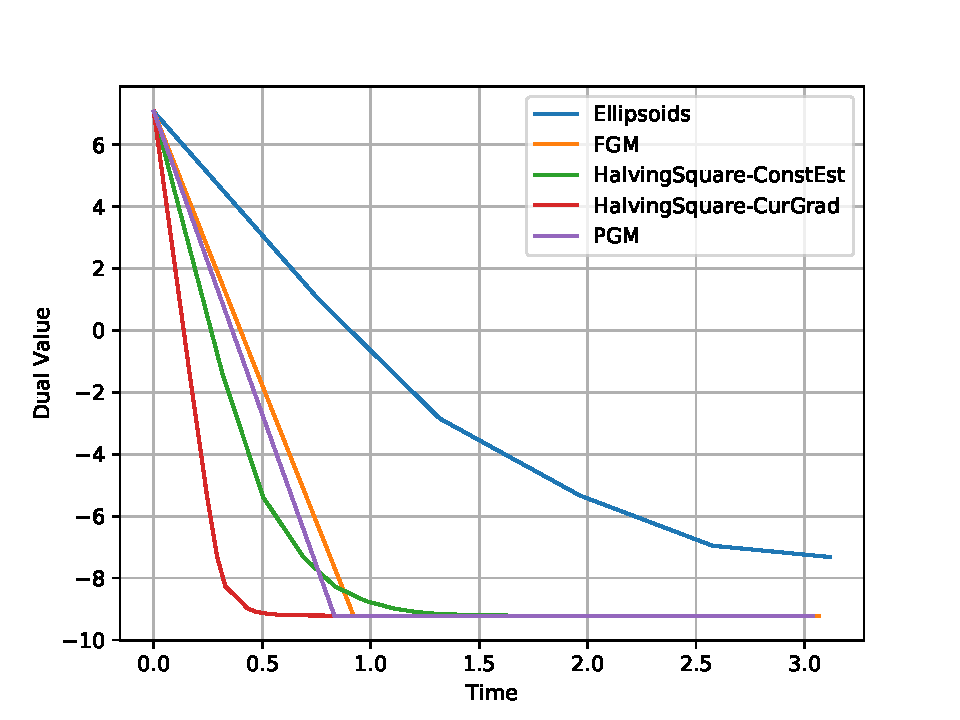
\includegraphics[width=0.25\linewidth]{Tests/Images/10_1e-01.pdf} \label{10_1} }  
\hspace{2ex}
\subfigure[]{
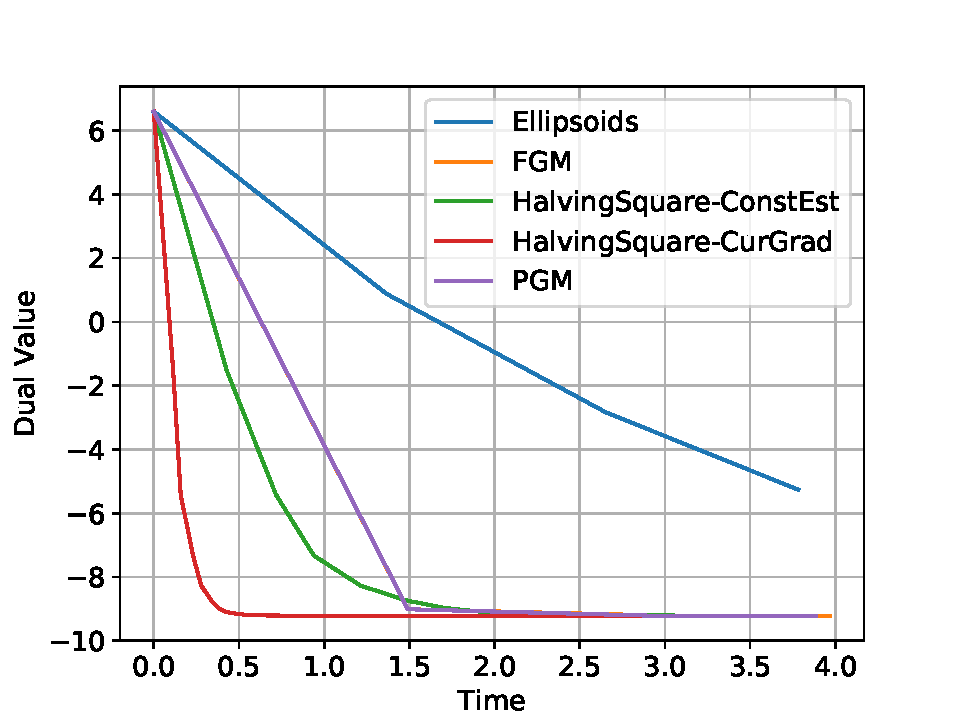
\includegraphics[width=0.25\linewidth]{Tests/Images/10_1e-03.pdf} \label{10_3} }
\hspace{2ex}
\subfigure[]{ \includegraphics[width=0.25\linewidth]{Tests/Images/10_1e-10.pdf} \label{10_10} }  
\vspace{2ex}
\subfigure[]{
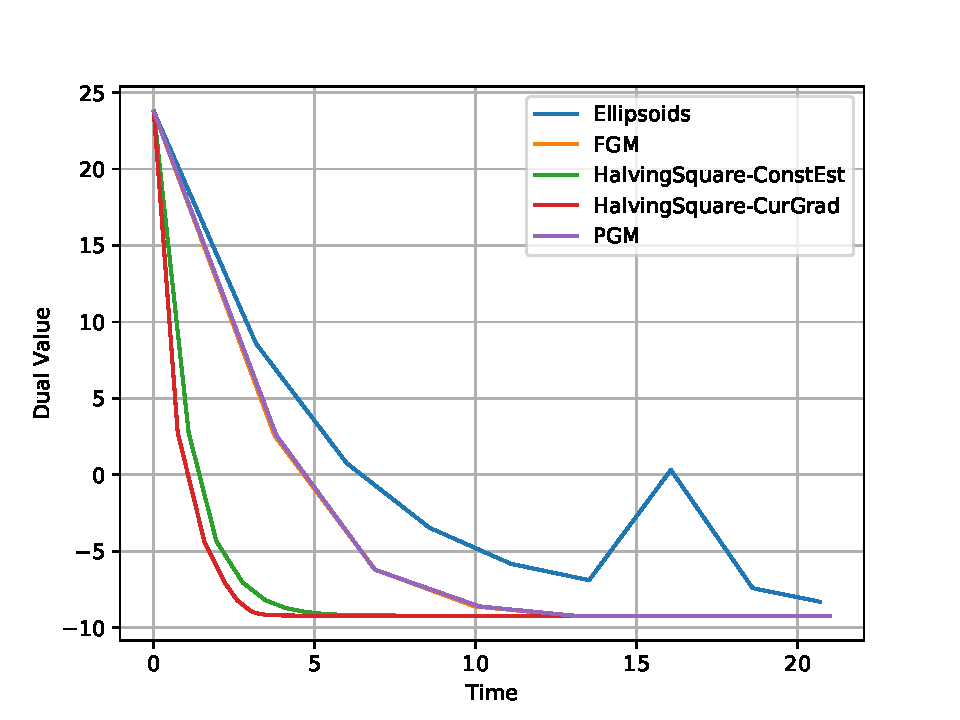
\includegraphics[width=0.25\linewidth]{Tests/Images/100_1e-01.pdf} \label{100_1} }  
\hspace{2ex}
\subfigure[]{
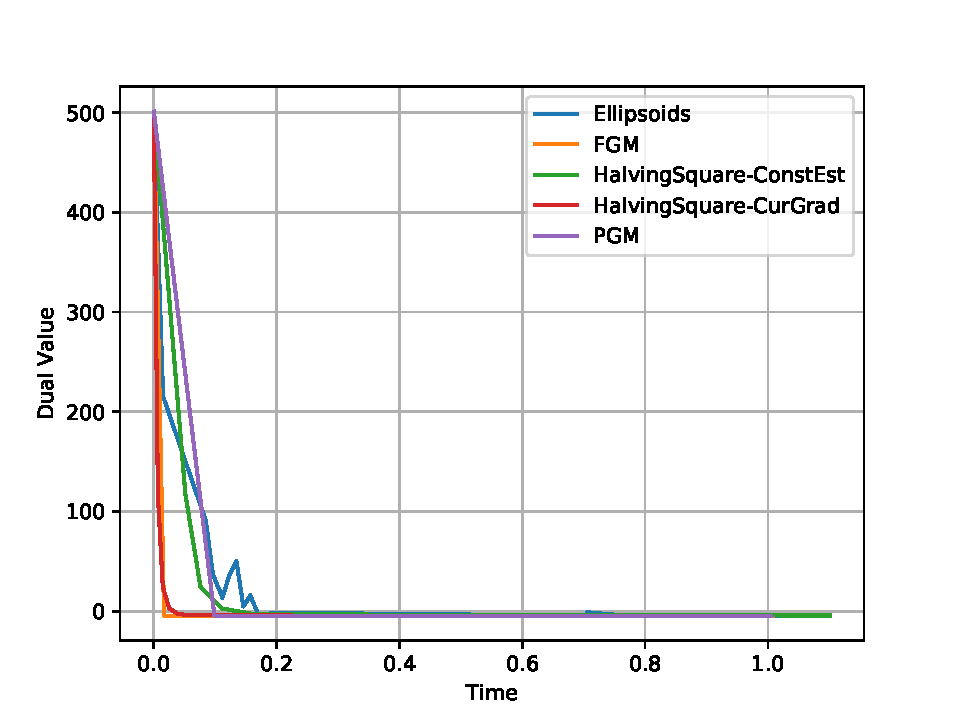
\includegraphics[width=0.25\linewidth]{Tests/Images/100_1e-03.pdf} \label{100_3} }
\hspace{2ex}
\subfigure[]{ 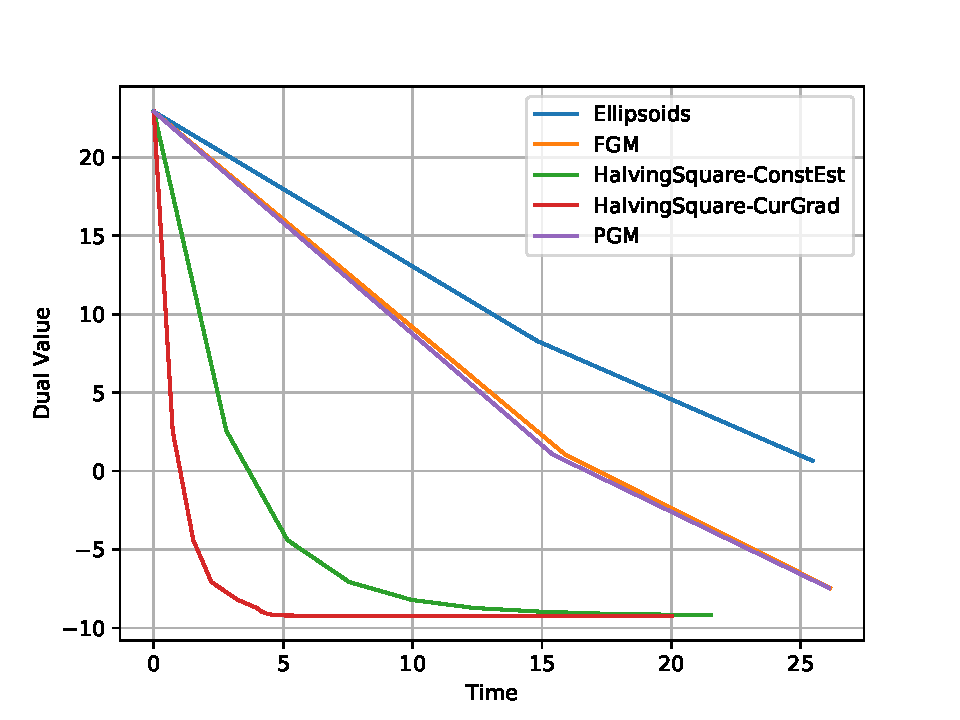
\includegraphics[width=0.25\linewidth]{Tests/Images/100_1e-10.pdf} \label{100_10} }
\caption{Comparison of different on inexact methods for task with different dimension $N$ and for different required accuracy $\epsilon$: \subref{10_1} $N=10,\epsilon=10^{-1}$; \subref{10_3} $N=10,\epsilon=10^{-3}$; \subref{10_10} $N=10,\epsilon=10^{-10}$; \subref{100_1} $N=10,\epsilon=10^{-1}$; \subref{100_3} $N=100,\epsilon=10^{-3}$; \subref{100_10} $N=100,\epsilon=10^{-10}$. } \label{fig:image}
\end{figure}

Let's compare our method with inexact ellipsoid method and primal gradient method with $(\delta, L,\mu)$ oracle (see previous subsection \ref{Inexact}) on a dual task.

For to find $\textbf{x}(\lambda)$ we will use gradients descent. There are theoretical result that can help to manange distance $\|\textbf{x}_k-\textbf{x}^*\|$ from current to optimal points. In particular, there are following results:
\begin{itemize}
\item If $f$ is a convex function with $L$-Lipschitz continious gradient then gradient descent with step $\alpha_k = \frac{1}{L}$ converges with speed
$$\|f(\textbf{x}_k)-f(\textbf{x}^*)\|\leq \frac{\|\textbf{x}_0-\textbf{x}^*\|}{k+4}$$
\item If $f$ is a $\mu$-strong convex function with $L$-Lipschitz continious gradient then gradient descent with step $\alpha_k = \frac{1}{L+\mu}$ converges with speed
$$\|f(\textbf{x}_k)-f(\textbf{x}^*)\|\leq \left(\frac{M-1}{M+1}\right)^kL\|\textbf{x}_0-\textbf{x}^*\|,$$
where $M =\frac{L}{\mu}$.
\end{itemize}
The proves for this statements one can find in many books of optimization, for example, in the book \cite{Polyak}. For all inexact method we will calculate $x(\lambda)$ with such accuracy as the method will converge to the solution with same for all methods accuracy $\epsilon$

We consider following prime task:

\begin{gather}
\label{prime}
f(\textbf{x}) = \ln \left(1+\sum_{k=1}^me^{\textbf{a}_k^\top\textbf{x}}\right) + C\|\textbf{x}\|_2^2\rightarrow \min\limits_{\textbf{x}}\\
\text{s.t.}\,\textbf{x}\in \mathbb{R}\\
g_k(\textbf{x}) = \textbf{b}_k^\top\textbf{x}-R_k\leq0, k = \overline{1,n}\\
\end{gather}

It is task of minimization the LogSumExp-function with $l2$-regularization. The regularization parameter $C$ determines strong convexity of our task and in the tests one takes $C$ equaled 1. The $N$ is diminsionality of primal task and is determined for different tests below. Matrixes $A = \|\textbf{a}_k\|_{k=1}^m \in\mathbb{R}^{n\times m}$ and $B = \|\textbf{b}_k\|_{k=1}^n \in\mathbb{R}^{N\times n}$ are being generated randomly. The $n$ is equal to dimensionality of dual task and in the current case is equal to 2. The $m$ is equal to 10 in our experiments and has not changes.

We introduce the following notation:

\begin{equation}
\label{phi}
\phi(\lambda_1, \lambda_2) = -\min\limits_{\textbf{x}}\left(f(\textbf{x}) +\lambda_1 g_1(\textbf{x}) +\lambda_2g_2(\textbf{x})\right)
\end{equation}

In such notations the dual task for the task \ref{prime} looks like:

\begin{gather}
\phi(\lambda_1, \lambda_2) \rightarrow \min\limits_{\lambda_1, \lambda_2}\\
\text{s.t}\, \lambda_1, \lambda_2 \geq 0
\end{gather}
 
Obviously, $\min\limits_{\textbf{x}}f(\textbf{x}) \geq 0$. Therefore, according to \ref{restr:dual} we can add following conditions on the dual variables:

$$|\lambda_k| \leq \lambda_{\text{max}}=\frac{f(\overline{\textbf{x}})}{\gamma}, k=1,2$$

And we have following task:

$$\phi(\lambda_1, \lambda_2) \rightarrow \min_{0\leq\lambda_k\leq\lambda_{max}}$$

How to calculate function and derivatave value for such task was discussed in the section \ref{details}.

We can see on \ref{fig:image} the following results. Firstly, the halving square method with provided in this work strategy \textbf{CurGrad} are the fastest method in the most tests tests. This method can be slower than other inexact methods if dimensional of primal task is small or $\epsilon$ is big. In particular, this strategy is faster than strategy with constant estimate provided in \cite{Ston_Pas}. It proves that provided by Nesterov method with strategy through gradient is the best method for to solve two dimensional dual task of minimization. Secondly, the gain of this strategy in comparison with other method is increase when the required $\epsilon$ decrease. This fact demonstrated important advantange of this strategy: it does not depend on required accuracy strongly. So, this method with constant estimate has strong dependity on it because there is this accuracy in the constant estimate, PGM and inexact ellipsoid method require that the $x(\lambda)$ is found with accuracy depended on $\epsilon$. But halving square with ellipsoid method has not such dependety.
\section{Conclusion}
\newpage
\begin{thebibliography}{3}
\bibitem{task}
Gasnikov A.  Universal gradient descent // MIPT --- 2018, 240 p.
\bibitem{Ston_Pas}
Pasechnyk D.A., Stonyakin F.S.  One method for minimization a convex Lipchitz continuous function of two variables on a fixed square // arXiv.org e-Print archive. 2018. – URL: \href{https://arxiv.org/pdf/1812.10300.pdf}{https://arxiv.org/pdf/1812.10300.pdf}
\bibitem{Nesterov}
Nesterov U.E.  Methods of convex optimization // M.MCNMO --- 2010, 262 p.
\bibitem{conda}
Anaconda[site]. At available: \href{https://www.anaconda.com}{https://www.anaconda.com}
\bibitem{DDR-theorem}
Danskin, J.M.: The theory of Max-Min, with applications. J. SIAM Appl. Math.14(4) (1966)
\bibitem{Stonykin}
Fedor S. Stonyakin, Mohammad S. Alkousa, Alexander A. Titov,and Victoria V. Piskunova1 On Some Methods for Strongly Convex Optimization Problems with One Functional Constraint // ...
\bibitem{PGM}
Olivier Devolder Exactness, Inexactness and Stochasticityin First-Order Methods for Large-ScaleConvex Optimization // UCL --- 2013,
\bibitem{Ellipsoids}
Need Reference To Book with Inexact Ellipsoids
\bibitem{Polyak}
B.T. Polyak. The Introduction to Optimization // Moscow, Science - 1983
\bibitem{my_git}
Repository with code: \href{https://github.com/ASEDOS999/Optimization-Halving-The-Square}{https://github.com/ASEDOS999/Optimization-Halving-The-Square}
\end{thebibliography}
\end{document}
